


%_______________
\section{Review exercises}

% 1

\eoce{\qt{Cleveland vs. Sacramento\label{cleveland_sacramento}} Average income varies 
from one region of the country to another, and it often reflects both 
lifestyles and regional living expenses. Suppose a new graduate is considering 
a job in two locations, Cleveland, OH and Sacramento, CA, and he wants to see 
whether the average income in one of these cities is higher than the other. He 
would like to conduct a hypothesis test based on two small samples from the 
2000 Census, but he first must consider whether the conditions are met to 
implement the test. Below are histograms for each city. Should he move forward 
with the hypothesis test? Explain your reasoning. \\
\begin{minipage}[c]{0.7\textwidth}
\begin{center}
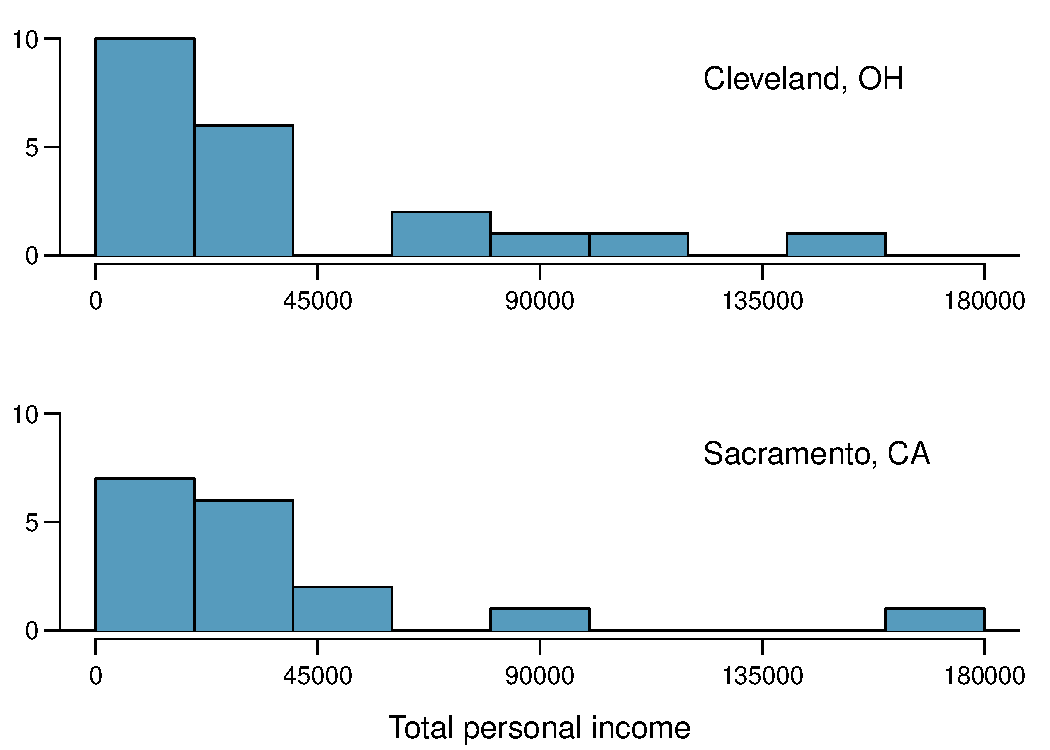
\includegraphics[width=0.95\textwidth]{ch_summarizing_data/figures/eoce/cleveland_sacramento/cleveland_sacramento_hist.pdf}
\end{center}
\end{minipage}
\begin{minipage}[c]{0.3\textwidth}
{\small
\begin{tabular}{l c}
\hline
        & Cleveland, OH \\
\hline
Mean    & \$ 35,749     \\
SD      & \$ 39,421     \\
n       & 21                
\end{tabular}

\vspace{2cm}

\begin{tabular}{l c}
\hline
        & Sacramento, CA \\
\hline
Mean    & \$ 35,500 \\
SD      & \$ 41,512 \\
n       & 17
\end{tabular}
}
\end{minipage}
}{}

% 2

\eoce{\qt{Oscar winners\label{oscar_winners}} The first Oscar awards for best actor 
and best actress were given out in 1929. The histograms below show the age 
distribution for all of the best actor and best actress winners from 1929 to 
2018. Summary statistics for these distributions are also provided. Compare the 
distributions of ages of best actor and actress winners.\footfullcite{data:oscars} \\
\begin{minipage}[c]{0.72\textwidth}
\begin{center}
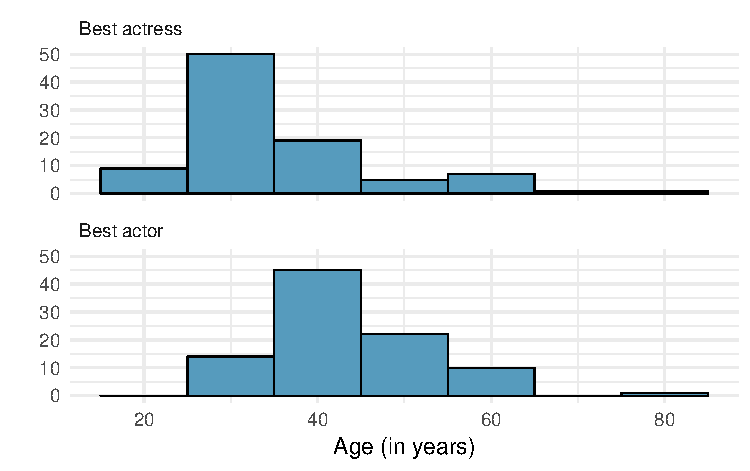
\includegraphics[width=0.95\textwidth]{ch_summarizing_data/figures/eoce/oscar_winners/oscars_winners_hist.pdf}
\end{center}
\end{minipage}
\begin{minipage}[c]{0.27\textwidth}
{\small
\begin{tabular}{l c}
\hline
        & Best Actress  \\
\hline
Mean    & 36.2      \\
SD      & 11.9      \\
n       & 92        \\  
        & \\
        & \\
        & \\
        & \\
        & \\
\hline
        & Best Actor \\
\hline
Mean    & 43.8 \\
SD      & 8.83 \\
n       & 92
\end{tabular}
}
\end{minipage}
}{}
